%%% Versao 1.0
%%% Data: Abril de 2015
%%% Autor: Cristiano Bertolini

%%% Definicao da classe para a proposta e artigo no padrao SBC
\documentclass[12pt,a4paper]{article}
\usepackage{upquote}
\usepackage{color}
\usepackage{graphicx,url}
\usepackage{graphicx}
\usepackage{hyperref} 
\usepackage{authblk}
\usepackage{fancyhdr}
\usepackage[brazil]{babel}   
\usepackage[T1]{fontenc}  
\usepackage{multirow}
\usepackage[table,xcdraw]{xcolor}
%\usepackage[utf8]{inputenc}
\usepackage{datetime} 
\usepackage{textcomp} 
 
%\usepackage{hyperref}
\usepackage[latin1]{inputenc}
%\input{macros.tex}  

%%%------------------SBC-ARTIGO--------------------------
%%% Pacote com o padrao SBC
\usepackage{sbc-template}
\usepackage{listings}
\renewcommand{\lstlistingname}{Algoritmo}

% CSS
\lstdefinelanguage{CSS}{
keywords={color,background-image:,margin,padding,font,weight,display,position,top,left,right,bottom,list,style,border,size,white,space,min,width,
transition:, transform:, transition-property, transition-duration,
transition-timing-function},
sensitive=true,
morecomment=[l]{//},
morecomment=[s]{/*}{*/},
morestring=[b]',
morestring=[b]",
alsoletter={:},
alsodigit={-}
}

% JavaScript
\lstdefinelanguage{JavaScript}{
morekeywords={typeof, new, true, false, catch, function, return,
null, catch, switch, var, if, in, while, do, else, case, break},
morecomment=[s]{/*}{*/},
morecomment=[l]//,
morestring=[b]",
morestring=[b]'
}

\lstdefinelanguage{HTML5}{
language=html,
sensitive=true,
alsoletter={<>=-},
morecomment=[s]{<!-}{-->},
tag=[s],
otherkeywords={
% General
>,
% Standard tags
<!DOCTYPE,
</html, <html, <head, <title, </title, <style, </style, <link,
</head, <meta, />,
% body
</body, <body,
% Divs
</div, <div, </div>,
% Paragraphs
</p, <p, </p>,
% scripts
</script, <script,
% More tags...
<canvas, /canvas>, <svg, <rect, <animateTransform, </rect>, </svg>,
<video, <source, <iframe, </iframe>, </video>, <image, </image>
},
ndkeywords={
% General
=,
% HTML attributes
charset=, src=, id=, width=, height=, style=, type=, rel=, href=,
% SVG attributes
fill=, attributeName=, begin=, dur=, from=, to=, poster=, controls=,
x=, y=, repeatCount=, xlink:href=,
% CSS properties
margin:, padding:, background-image:, border:, top:, left:,
position:, width:, height:,
% CSS3 properties
transform:, -moz-transform:, -webkit-transform:,
animation:, -webkit-animation:,
transition:, transition-duration:, transition-property:,
transition-timing-function:,
}
}

\lstset{%
% Basic design
% backgroundcolor=\color{lightgray},
basicstyle={\small\ttfamily},
frame=l,
% Line numbers
xleftmargin={0.75cm},
numbers=left,
stepnumber=1,
firstnumber=1,
numberfirstline=true,
% Code design
identifierstyle=\color{black},
keywordstyle=\color{blue}\bfseries,
ndkeywordstyle=\color{green}\bfseries,
 stringstyle=\color{red}\ttfamily,
commentstyle=\color{darkgray}\ttfamily,
% Code
language={HTML5},
tabsize=2,
showtabs=false,
showspaces=false,
captionpos=b,
showstringspaces=false,
extendedchars=true,
breaklines=true
}


%%%% Titulo, autores e identificacao no padrao SBC
\sloppy
%%% Colocar o titulo do seu trabalho 
\title{Um Processo de Classifica��o de Regras de Acessibilidade Web}
%%% colocar o seu nome seguido do co-orientador (se existir) e orientador
\author{Carine Piovesan Lopes, Cristiano Bertolini, Guilherme Bernardino da Cunha }

\address{Universidade Federal de Santa Maria - UFSM\\
 Centro de Educa��o Superior Norte - CESNORS, Frederico Westphalen, RS 
  \email{carinepiovesan@gmail.com, cristiano.bertolini@ufsm.br,
  guilherme@ufsm.br}}
 
%%%------------------SBC-ARTIGO-------------------------- 

\begin{document}

%%% Para o artigo vc deve incluir o comando abaixo
\maketitle 

%%%-----------------------------------%% BEGIN ARTIGO
% %\begin{abstract}
%Here goes the abstract\ldots
%\end{abstract}
 
 \begin{resumo}
O desenvolvimento web tem evoluido nos �ltimos anos, desta forma
aumentaram as preocupa��es em manter o conte�do dispon�vel � todos os
usu�rios. A acessibilidade web � a flexibiliza��o do acesso �s informa��es a
todos os usu�rios independente de suas limita��es e necessidades. Atualmente, 
v�rias ferramentas para verifica��o de acessibilidade est�o dispon�veis, por�m
muitas delas se sobrep�em, deixando a d�vida de qual seria a mais completa
para utiliz��o visto que as mesmas n�o especificam quais recomenda��es s�o
verificadas por elas. Este artigo apresenta um processo de classifica��o das
regras de acessibilidade web baseado nas recomenda��es de acessibilidade
brasileira o E-MAG (Modelo de Acessibilidade em Governo Eletr�nico).
A classifica��o das regras consiste na an�lise das recomenda��es e classifica��es
em regras sint�ticas e sem�nticas. As regras sint�ticas poder�o ser testadas e
verificadas de forma autom�tica, dando maior agilidade ao processo de
verifica��o de acessibilidade, enquanto que as regras sem�nticas s�o aquelas
que necessitam de testes e verifica��es manuais. Um estudo
de caso foi realizado, atrav�s da utiliza��o de uma
ferramenta de verifica��o de acessiblidade aplicado � p�ginas
iniciais de sites relacionados ao governo brasileiro para que o processo
proposto neste trabalho pudesse ser validado.
Acredita-se que esta classifica��o possa dar mais agilidade no processo de verifica��o de
acessibilidade e ajudar no desenvolvimento de websites
acess�veis.

%\ldots
\end{resumo}
  
 \section{Introdu��o}
\label{sec:introducao}
 
O crescimento e desenvolvimento das tecnologias de informa��o no decorrer dos
�ltimos anos vem causando impactos na vida pessoal e profissional das
pessoas. A utiliza��o da web nos dias atuais � importante, tanto para neg�cios e
estudos como para entretenimento. Conforme dados obtidos atrav�s de pesquisas
do PNAD (IBGE), no ano de 2013, 49,6\% da popula��o brasileira, correspondente a
85,6 milh�es de pessoas com idade superior a 10 anos j� possu�a o acesso �
internet~\cite{IBGE}.

O desenvolvimento web pode ser representado como uma evolu��o do desenvolvimento
de software convencionais, promovendo assim, preocupa��es adicionais
relacionadas a seu desenvolvimento, mantendo como objetivo a aplica��o dos
princ�pios da engenharia de software para que se obtenha
qualidade~\cite{Pressman}. O foco est� em desenvolver aplica��es corretas e
completas de acordo com os requisitos de seus usu�rios, considerando a
infraestrutura onde ser� executada e disponibilizada. 

Segundo Hewet~\cite{Hewett}, Intera\c{c}\~ao
Humano Computador \'e uma disciplina ligada ao projeto, implementa\c{c}\~ao e
avalia\c{c}\~ao de sistemas computacionais interativos usados pelo ser humano,
juntamente com os fen\^omenos ocorridos relacionado a este uso. 
Inicialmente o conceito de intera\c{c}\~ao tratava de uma s\'erie de est\'imulos
que devolviam respostas. Com o surgimento das pesquisas cognitivas, passou-se
a enfatizar intera\c{c}\~ao como sendo a comunica\c{c}\~ao com
m\'aquinas~\cite{Card}.Recentemente o conceito de intera\c{c}\~ao, baseia-se na
comunica\c{c}\~ao intermediada por sistemas de computadores. Sendo assim podemos
considerar uma intera\c{c}\~ao como um processo de
comunica\c{c}\~ao~\cite{Barbosa}.

A acessibilidade � um processo din�mico associado n�o s� ao desenvolvimento
tecnol�gico mas principalmente ao desenvolvimento da sociedade, um conceito que
envolve tanto aspectos f�sicos quanto o espa�o digital~\cite{Torres}. A
acessibilidade Web pode ser obtida atrav�s das normas existentes nas diretrizes
de acessibilidade fornecidas pela W3C ou no caso do Brasil o \emph{Checklist}
E-MAG~\cite{eMAG,LAI}.
    
Apesar da exist�ncia de diversas diretrizes de acessibilidade e leis federais
tais como a Lei N�10.048 que define acessibilidade ao fato de estar relacionada
em fornecer condi��o para utiliza��o, com seguran�a e autonomia, total ou
assistida, dos espa�os, mobili�rios e equipamentos urbanos, das edifica��es, dos
servi�os de transporte e dos dispositivos, sistemas e meios de comunica��o e
informa��o, por pessoa com defici�ncia ou com mobilidade reduzida, muitos
portais ainda possuem grandes limita��es e barreiras a algum determinado grupo
de usu�rios~\cite{Freire,AcessibilidadeBrasil}.  

Segundo o N�cleo de Acessibilidade da
UFSM\footnote{http://w3.ufsm.br/acessibilidade/}, em um levantamento realizado,
entre os anos de 2008 e 2014 foram constatados 255(1,03\%) estudantes com
defici�ncia ingressos nos diferentes Campus da Universidade atrav�s da cota B.
Destes, 90 (35,29\%) estudantes abandonaram seu curso, 24 (9,41\%) estudantes
conclu�ram seu curso e 141 (55,29\%) estudantes est�o em situa��o regular. 

Atualmente, al�m das diretrizes de acessibilidade para conte�do web (WCAG) 2.0
que abrangem uma grande variedade de recomenda��es para tornar o conte�do web
acess�vel~\cite{Caldwell}, encontramos tamb�m v�rias ferramentas para
verifica��o de acessibilidade, que podem contribuir para o desenvolvimento de
uma web acess�vel.

Segundo Freire~\cite{Freire}, as ferramentas para verifica��o e valida��o de
acessibilidade web contribuem muito no aux�lio aos desenvolvedores principalmente aos problemas
relacionados � marca��o. Estas ferramentas disp�em de muitas fun��es que ajudam
desenvolvedores no aux�lio de detec��o e reparo dos problemas
encontrados. Kelly \emph{et al.}~\cite{Kelly} apresenta que um determinado site
validado pelos n�veis de prioridade da W3C (A, AA, AAA), quando testados por
usu�rios com limita��es, n�o obteve um grau de 100\% de acessibilidade. Ao final
da pesquisa concluiu-se que alguns dos problemas encontrados pelos usu�rios,
n�o haviam sido considerados pelos avaliadores autom�ticos, mesmo seguindo as
Diretrizes da W3C e WCAG 2.0.

Este trabalho prop�e um processo de classifica��o de regras das recomenda��es de
acessibilidade web do documento brasileiro E-MAG (Modelo de Acessibilidade em
Governo Eletr�nico), podendo ser aplicado tamb�m ao modelo internacional, da
W3C o WCAG (Web Content Accessibility Guidelines: Recomenda��es de
Acessibilidade para Conte�do Web). Atrav�s desta classifica��o � poss�vel
observar e apontar quais regras podem ser verificadas e testadas de modo
automatizado e quais regras podem ser verificadas e testadas de modo manual, a
fim de contribuir para uma verifica��o mais r�pida e espec�fica da melhor
forma poss�vel, ``visto que a promo��o da acessibilidade de sistemas
computacionais interativos para uso humano est� diretamente relacionada ao
exerc�cio da cidadania''~\cite{Melo}. Ap�s a classifica��o de regras do
documento E-MAG, foi tamb�m aplicado um estudo de caso em paginas
governamentais a fim de validar a classifica��o das regras realizada.


Este trabalho est� organizado da seguinte forma: a
Se��o~\ref{sec:referencialTeorico} apresenta o referencial te�rico do trabalho;
Se��o~\ref{sec:processoDeClassificacao} apresenta o processo de classifica��o; a
Se��o~\ref{sec:geracaoDeRegrasDeAcessibilidade} apresenta a gera��o das regras
de acessibilidade; a
a Se��o~\ref{sec:trabalhosRelacionados} apresenta os trabalhos relacionados; a
a Se��o~\ref{sec:conclusoes} apresenta as
conclus�es e as refer�ncias bibliogr�ficas. 
 \section{Referencial Te\'orico}
\label{sec:referencialTeorico}


\subsection{Acessibilidade Web}
\label{subsec:AcessibilidadeWeb}

Nos \'ultimos anos, o desenvolvimento Web teve um grande crescimento visto que
a intera\c{c}\~ao com a Web vem se tornando comum no dia a dia das pessoas, seja para
trabalho, estudo ou entretenimento. Ao fazer um retrospecto da Web, podemos
visualizar um grande avan\c{c}o, pois passamos de p\'aginas est\'aticas para o
processamento de p\'aginas mais interativas e din\^amicas, permitindo agregar
facilidades e uma grande gama de recursos para disponibiliza\c{c}\~ao do
conte\'udo~\cite{Jazayeri}.Assim, tem-se criado diversos m\'etodos de suporte
para os desenvolvimentos de aplica\c{c}\~oes Web acess\'iveis~\cite{Freire}.

Apesar dos v\'arios m\'etodos pra aplica\c{c}\~ao de desenvolvimento de uma web
mais acess\' ivel, ainda encontramos dificuldades na implementa\c{c}\~ao da
cultura de acessibilidade, pois os desenvolvedores ainda n\~ao se conscientizaram sobre a
import\^ancia do tema Web Acess\'ivel. A implanta\c{c}\~ao de acessibilidade
demanda conhecimentos sobre a vantagem e desvantagem de cada m\'etodo a ser implementado,
exigindo muito estudo~\cite{Freire}.    
 
Segundo a W3C~\cite{WAI}, para que um site possa ser desenvolvido de forma
acess\'ivel, \'e necess\'ario que v\'arios componentes estejam interligados, muitos recursos de
acessibilidade podem ser implementados facilmente, desde que no in\'icio do
desenvolvimento do projeto sejam identificados os problemas que impedem a
acessibilidade web. Componentes estes que abrangem conte\'udo, c\'odigos de
marca\c{c}\~ao, ferramentas de cria\c{c}\~ao, desenvolvedores, tecnologias
espec\'ificas para cada defici\^encia quando necess\'ario, entre outros.

A W3C, organiza\c{c}\~ao que padroniza a web,
determina que acessibilidade web permite que diferentes usu\'arios tenham eles
qualquer tipo de defici\^encia tais como auditiva, cognitiva, visual,
f\'isica, de fala, entre outras, possam utilizar a Web e o conte\'udo nela
disponibilizada, ou seja, que possam perceber, compreender, interagir enavegar
na Web independente de suas habilidades e defici\^encias~\cite{WAI/W3C}.

O governo Brasileiro tamb\'em mostra muito interesse quando falamos em
acessibilidade web, podemos visualizar tal interesse quando no decreto N\textsuperscript{\underline{o}} 5.296
de 2 de dezembro de 2004. O governo determina o regulamento das Leis
N\textsuperscript{\underline{o}} 10.048, de 8 de novembro de 2000, e 10.098, de
19 de dezembro de 2000. Segundo o governo brasileiro acessibilidade se refere
\`a utiliza\c{c}\~ao total de todos os recursos fornecidos em qualquer \'area,
excluindo poss\'iveis barreiras que venham a limitar o acesso a qualquer pessoa~\cite{AcessibilidadeBrasil}. 

A \emph{Lei de Acesso \`a Informa\c{c}\~ao} N\textsuperscript{\underline{o}} 12.527/2011 regulamenta o
direito constitucional de acesso \`as informa\c{c}\~oes p\'ublicas. A norma entrou em vigor em
16 de maio de 2012 criando mecanismos que possibilitam, a qualquer pessoa, 
f\'isica ou jur\'idica, sem necessidade de apresentar motivo, o recebimento de
informa\c{c}\~oes p\'ublicas dos \'org\~aos e entidades. A lei vale para os
tr\^es Poderes da Uni\~ao, Estados, Distrito Federal e Munic\'ipios, inclusive aos
Tribunais de Conta e Minist\'erio P\'ublico. Entidades privadas sem fins
lucrativos tamb\'em s\~ao obrigadas a dar publicidade a informa\c{c}\~oes referentes
ao recebimento e \`a destina\c{c}\~ao dos recursos p\'ublicos por elas
recebidos~\cite{LAI}.


\subsection{Padr\~oes de Acessibilidade Web}
\label{subsec:PadroesdeAcessibilidadeWeb}
 
As diretrizes de Acessibilidade para Conte\'udo Web (WCAG) 2.0, sucede a WCAG
1.0 que foi criado em 1999, abrangem uma grande variedade de recomenda\c{c}\~oes
que faz com que a web e seu conte\'udo sejam mais acess\'iveis \`as pessoas que
tenham algum tipo de defici\^encia, neste documento podemos encontrar afirma\c{c}\~oes que
podem ser testadas sem algum tipo de tecnologia espec\'ifica~\cite{Caldwell}. 

A WCAG 2.0 aborda quatro n\'iveis importantes para ajudar desenvolvedores e
organiza\c{c}\~oes a proporcionar ao seu p\'ublico alvo um conte\'udo mais
acess\'ivel \`a todos os tipos de usu\'arios, s\~ao estes os n\'iveis abordados
na vers\~ao WCAG 2.0:

\begin{itemize}
  \item \textbf{Princ\'ipios:} fornecem a base para um conte\'udo Web
  acess\'ivel na qual se enquadram as caracter\'isticas percept\'ivel, oper\'avel,
  compreens\'ivel e robusto;
  \item \textbf{Diretrizes:} fornecem informa\c{c}\~oes de como deixar o
  conte\'udo web mais acess\'ivel a usu\'arios com diferentes defici\^encias.
  \item \textbf{Crit\'erios de Sucesso:} s\~ao atribu\'idos a cada diretriz
  tr\^es n\'iveis de conformidade ou prioridade A, AA e AAA utilizados para
  satisfazer diferentes situa\c{c}\~oes encontradas durante o processo de
  desenvolvimento. Prioridade A: determina pontos nas quais os desenvolvedores
  Web DEVEM satisfazer inteiramente, Prioridade AA: Pontos nas quais os
  desenvolvedores DEVERIAM satisfazer, Prioridade AAA: Pontos nas quais os
  desenvolvedores PODEM satisfazer;
  \item \textbf{T\'ecnicas de tipo Necess\'aria e de tipo Sugerida:} s\~ao
  t\'ecnicas de testes necess\'arios para cumprir os crit\'erios de sucesso ao
  aplicar as recomenda\c{c}\~oes estabelecidas pela WCAG 2.0 e as t\'ecnicas de tipo
  sugerido s\~ao aquelas nas quais poderiam ser aplicados t\'ecnicas de testes
  \`as recomenda\c{c}\~oes, por\'em estas n\~ao s\~ao abrangidas pelos crit\'erios
  de sucesso test\'aveis~\cite{Caldwell}.
\end{itemize} 

O Modelo de Acessibilidade em Governo Eletr\^onico (E-MAG) \'e o modelo de
diretriz de acessibilidade brasileiro e  tem como compromisso, ser o norteador de
acessibilidade Web nos portais federais brasileiros, garantido o acesso as
informa\c{c}\~oes neles disponibilizados por toda a popula\c{c}\~ao~\cite{eMAG}.  
     
O E-MAG possui recomenda\c{c}\~oes de acessibilidade conforme as necessidades
brasileiras e em conformidade com os padr\~oes de diretrizes internacionais
(WCAG),o documento \'e dividido em seis diretrizes que seguem as
recomenda\c{c}\~oes de acessibilidade determinadas pela WCAG 2.0, s\~ao elas:

\begin{itemize}
  \item \textbf{Marca\c{c}\~ao:} \'e constitu\'ida por recomenda\c{c}\~oes que
  se referem ao cumprimento e respeito dos padr\~oes Web, envolvendo a pr\'atica da organiza\c{c}\~ao do
  c\'odigo e sua sem\^antica. 
  \item \textbf{Comportamento (Document Object Model - DOM):} constitu\'ida por
  recomenda\c{c}\~oes quanto aos comandos e meios de acesso as p\'aginas por
  meio do teclado.  
  \item \textbf{Conte\'udo/Informa\c{c}\~ao:} refere-se \`a recomenda\c{c}\~oes
  que dizem respeito ao conte\'udo disponibilizado pelo site, tais como idioma principal, t\'itulos
  descritivos, descri\c{c}\~ao de imagens garantia de entendimento do conte\'udo
  por todos os tipos de usu\'arios.  
  \item \textbf{Multim\'idia:} refere-se \`a recomenda\c{c}\~oes que dizem
  respeito aos v\'arios meios de transmitir as informa\c{c}\~oes e conte\'udos em formatos
  multim\'idia, sejam elas por v\'ideos, \'audios, anima\c{c}\~oes e
  audiodescri\c{c}\~oes.
  \item \textbf{Formul\'ario (E-MAG, 2014):} refere-se \`a recomenda\c{c}\~oes
  que dizem respeito aos formul\'arios, tais como reconhecimentos de erros dos dados de
  entrada e confirma\c{c}\~oes de envio dos dados, estrat\'egias de
  seguran\c{c}a para substitui\c{c}\~ao do CAPTCHA~\cite{eMAG}.  
\end{itemize}
 
 Atualmente encontramos a especifica\c{c}\~ao WAI-ARIA
 (Accessible Rich Internet Applications Suite),na qual \'e uma
 recomenda\c{c}\~ao que trata de acessibilidade em interfaces ricas. A ARIA ajuda em conte\'udos 
 din\^amicos e controles avan\c{c}ados de interface, focando principalmente
 em usu\'arios que dependam de leitores de tela e usu\'arios que n\~ao possam
 utilizar o mouse~\cite{W3C}, é importante salientar que neste trabalho não
 esta sendo considerada esta especificação.


%Sommerville~\etal~\cite{Barbosa} e Wessberg~\cite{wessberg2000real}
 \section{Processo de Classifica��o}
\label{sec:processoDeClassificacao}


Foi proposto um processo de classifica��o que visa dividir as recomenda��es
em duas categorias sendo elas: sint�tica e sem�ntica. A categoria sint�tica contar� com
as regras que poder�o ser verificadas ao m�ximo poss�vel automaticamente, sem
interfer�ncia de testes humanos, enquanto que a categoria sem�ntica
por sua vez necessitar� de testes humanos.

\begin{figure}[!h]
\centering 
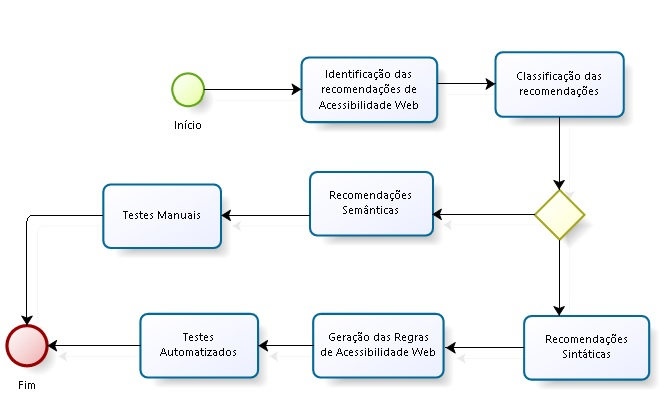
\includegraphics[scale=0.7]{figuras/processo3.jpg}  
\caption{Processo de Classifica��o Proposto}
\label{figura1}
\end{figure} 

A Figura~\ref{figura1} apresenta o modelo proposto para o processo de
classifica��o das recomenda��es de acessibilidade web. Este processo pode ser
considerado gen�rico, pois o mesmo pode ser aplicado a todos os websites, visto
que o mesmo tem o objetivo de realizar a verifica��o de acessibilidade web.  As
etapas do processo s�o:

\begin{itemize}
  
  \item \textbf{Identifica��o das Recomenda��es de Acessibilidade Web:} ser�o
  identificadas as recomenda��es de acessibilidade web descritas pelo E-MAG.
  
  \item \textbf{Classifica��o das Recomenda��es:} consiste na an�lise de cada
  recomenda��o e a divis�o das mesmas em duas partes que s�o elas regras
  sem�nticas e regras sint�ticas, essas regras formam um padr�o para a
  classifica��o no quesito de acessibilidade web.
  
  \item \textbf{Regras Sem�nticas:} as regras sem�nticas tratam do significado
  da estrutura de c�digo, o que verifica se o c�digo esta funcionando
  corretamente, mas n�o se esta escrito na forma correta.
  
  \item \textbf{Testes Manuais:} as regras sem�nticas necessitam de testes e
  corre��es com interven��o humana, j� que possuem um grande n�vel de
  complexidade na sua implementa��o.
  
   \item \textbf{Regras Sint�ticas:} as regras sint�ticas tratam da escrita e da
  valida��o dos c�digos HTML e CSS, a fim de verificar se os elementos do
  c�digo est�o sendo utilizadas para sua verdadeira finalidade.
  
   \item \textbf{Gera��o das Regras de Acessibilidade Web:} para cada
  recomenda��o de acessibilidade existente analisada e poss�vel de
  implementa��o, ser�o geradas as regras.
  
  \item \textbf{Testes Automatizados:} as regras sint�ticas podem ser
  automatizadas, ou seja, podem ser verificadas pelas ferramentas de
  verifica��o de acessibilidade e valida��o de c�digos HTML e CSS, sendo que
  verificam se o c�digo esta sendo utilizado de forma correta.
  
\end{itemize}



O Algoritmo~\ref{code1} apresenta um exemplo de c�digo HTML onde
sintaticamente � poss�vel verificar a recomenda��o
N\textsuperscript{\underline{o}} 1 do EMAG referente � Marca��o, que diz o
seguinte: \emph{Respeitar os Padr�es de Desenvolvimento Web}, baseada nos
crit�rios de Sucesso 4.1.1 e 4.1.2 do WCAG. 
Envolve especifica��es estabelecidas pela W3C, utilizadas para criar e
interpretar o conte�do web, tratando-se da linguagem de marca��o HTML. Essas tecnologias s�o
desenvolvidas prevendo a acessibilidade desses documentos ao maior grupo de indiv�duos poss�vel. Esta
recomenda��o chama a aten��o para a declara��o correta do DOCTYPE dos documentos
HTML e XHTML sendo que o mesmo informa qual a  vers�o do HTML esta sendo
utilizada, informa��o preciosa para que as ferramentas de valida��o possam
realizar a an�lise e indicar as corre��es.

\begin{lstlisting}[caption={Exemplo de DOCTYPE em HTML},label=code1]
<!DOCTYPE HTML PUBLIC "-//W3C//DTD HTML 4.01//EN"
 "http://www.w3.org/TR/html4/strict.dtd">
<html lang="pt-BR">
<head> 
<title>Exemplo de DOCTYPE em HTML 4.01</title> 
<meta http-equiv="content-type" content="text/html; charset=utf-8" />
</head>
\end{lstlisting}

Esta recomenda��o que estabelece o respeito aos padr�es web pode ser
considerada uma recomenda��o capaz de gerar v�rias regras, considerando a
exist�ncia de v�rios padr�es de desenvolvimento para cada tecnologia. Isso
envolve codificar as p�ginas web de acordo com as especifica��es t�cnicas de
cada tecnologia, de modo que as p�ginas produzidas possam ser interpretadas adequadamente.

Na vers�o do HTML 5 n�o � necess�ria a declara��o da sua vers�o, 
por�m h� a necessidade da declara��o do DOCTYPE, permitindo que as 
ferramentas de verifica��o e valida��o identifiquem o tipo de documento
analisado. Baseado no Algoritmo~\ref{code1}, o mesmo n�o seria acess�vel caso
as linhas 1 e 2 n�o estivessem escritas. No entanto, considerando apenas as
linhas 3 a 7, funcionariam normalmente possibilitando o acesso � qualquer
pessoa sem necessidades especiais.
 
Esta recomenda��o � de n�vel de prioridade A, ou seja, os desenvolvedores devem
atend�-la para que as tecnologias de apoio possam fazer a interpreta��o correta
das informa��es da p�gina web. Caso as declara��es n�o estejam corretas as
tecnologias de apoio correm o risco de n�o interpretar o conte�do ali existente
ou fazer a interpreta��o incorreta passando aos usu�rios informa��es n�o confi�veis.

Um exemplo de classifica��o sem�ntica � a recomenda��o N\textsuperscript{\underline{o}} 20
do E-MAG:  \emph{Fornecer alternativa em texto para imagens do web site},
baseado nos Crit�rios de Sucesso 1.1.1 do WCAG. O texto alternativo, como o nome j� diz,
� uma alternativa aos elementos n�o-textuais de uma p�gina web. A utiliza��o
correta desta recomenda��o, n�o depende unicamente do conhecimento de c�digo e
da utiliza��o de ferramentas mas sim do conhecimento humano, sensibilidade e interpreta��o
pessoal do profissional que inseriu a imagem na p�gina. Atualmente os sistemas e
leitores de tela n�o t�m a capacidade de interpretar imagens no contexto da
p�gina web, por isso � necess�rio que os textos alternativos permitam, por
exemplo, a tradu��o do conte�do da imagem pelos leitores de tela utilizados
por pessoas portadoras de defici�ncia visual.

O Algoritmo~\ref{code2} apresenta como o texto alternativo representado
atrav�s do atributo ALT, que deve estar inserido dentro do elemento IMG.
Toda imagem deve conter o atributo ALT mesmo que seja vazio ou nulo.
Quando o leitor de tela encontra uma imagem sem o atributo ALT, o mesmo extrai
informa��es sobre a imagem de outros lugares tais como o nome da imagem e
localiza��o, o que n�o determina a fun��o e especifica��o correta da imagem.

\begin{lstlisting}[caption={Exemplo de descri��o �s imagens},label=code2] 
<img src="foto-porto-alegre.jpg" alt="Foto de uma bicicleta de carga verde com
caixas laranjas encostada numa parede" />

\end{lstlisting}



 \section{Gera��o de Regras de Acessibilidade}

\label{sec:geracaoDeRegrasDeAcessibilidade} 

Baseada na classifica��o das recomenda��es contidas no modelo
E-MAG, para cada recomenda��o foram geradas regras. Esta classifica��o segue a
identifica��o num�rica descrita no modelo E-MAG~\cite{eMAG}.

A Tabela~\ref{tabelageracaoregras} apresenta as regras sint�ticas e sem�nticas. Os
problemas sint�ticos s�o de tratamento mais simples que os sem�nticos, a sintaxe
trata da verifica��o gramatical dos programas, ou seja, manipula os c�digos sem considerar os seus
significados. A sem�ntica necessita de an�lise da estrutura do c�digo pois
objetiva dar uma interpreta��o para a linguagem e interpreta��o do c�digo,
contendo alto n�vel de complexidade~\cite{Blauth}.

 
%tabelacompletaregras
% Please add the following required packages to your document preamble:
% \usepackage{multirow}
\begin{table}[]
\scriptsize
\caption{Classifica��o das regras do E-MAG}
\label{tabelageracaoregras}
\begin{tabular}{|l|l|l|l|}
\hline
\multirow{2}{*}{ID} & \multicolumn{1}{c|}{\multirow{2}{*}{Nome}}                                              & \multicolumn{2}{c|}{Classifica��o}                              \\ \cline{3-4} 
                    & \multicolumn{1}{c|}{}                                                                   & \multicolumn{1}{c|}{Sint�tica} & \multicolumn{1}{c|}{Sem�ntica} \\ \hline
1.1                 & Respeitar os Padr�es Web                                                                & X                              &                                \\ \hline
1.2                 & Organizar o c�digo HTML de forma l�gica e sem�ntica                                     & X                              &                                \\ \hline
1.3                 & Utilizar corretamente os n�veis de cabe�alho                                            & X                              & X                              \\ \hline
1.4                 & Ordenar de forma l�gica e intuitiva a leitura e tabula��o                               & X                              & X                              \\ \hline
1.5                 & Fornecer �ncoras para ir direto a um bloco de conte�do                                  & X                              & X                              \\ \hline
1.6                 & N�o utilizar tabelas para diagrama��o                                                   & X                              & X                              \\ \hline
1.7                 & Separar Links adjacentes                                                                & X                              &                                \\ \hline
1.8                 & Dividir �reas de informa��o                                                             & X                              &                                \\ \hline
1.9                 & N�o abrir novas inst�nias sem a solicita��o do usu�rio                                  & X                              &                                \\ \hline
2.1                 & Disponibilizar todas as fun��es via teclado                                             &                                & X                              \\ \hline
2.2                 & Garantir que os objetos program�veis sejam acess�veis                                   & X                              & X                              \\ \hline
2.3                 & N�o criar p�ginas  com atualiza��o autom�tica peri�dica                                 & X                              &                                \\ \hline
2.4                 & N�o criar redirecionamento autom�tico de p�ginas                                        & X                              &                                \\ \hline
2.6                 & N�o incluir situa��es com intermit�ncia de tela                                         &                                & X                              \\ \hline
3.1                 & Identificar o idioma principal da p�gina                                                & X                              & X                              \\ \hline
3.2                 & Informar mudan�as de idioma no conte�do                                                 &                                & X                              \\ \hline
3.3                 & Oferecer um t�tulo descritivo e informativo � p�gina                                    & X                              & X                              \\ \hline
3.5                 & Descrever links clara e sucintamente                                                    &                                & X                              \\ \hline
3.6                 & Fornecer alternativa em texto para imagens do site                                      & X                              & X                              \\ \hline
3.7                 & Utilizar mapas de imagens de forma acess�vel                                            &                                & X                              \\ \hline
3.8                 & Disponibilizar documentos em formatos acess�veis                                        &                                & X                              \\ \hline
3.9                 & Em tabelas, utilizar t�tulos e resumos de forma apropriada                              & X                              & X                              \\ \hline
3.10                & Associar c�lulas de dados �s c�lulas de cabe�alho                                       & X                              &                                \\ \hline
3.11                & Garantir a leitura e compreens�o das informa��es                                        &                                & X                              \\ \hline
3.12                & Disponibilizar uma explica��o para siglas,abreviaturas e palavras incomuns              &                                & X                              \\ \hline
4.1                 & Oferecer contraste m�nimo entre plano de fundo e primeio plano                          &                                & X                              \\ \hline
4.2                 & N�o utilizar apenas cor ou outras caracter�sticas sensoriais para diferenciar elementos &                                & X                              \\ \hline
4.3                 & Permitir redirecionamento sem perda de funcionalidade                                   &                                & X                              \\ \hline
4.4                 & Possibilitar que o elemento em foco seja visualmente evidente                           & X                              &                                \\ \hline
5.1                 & Fornecer alternativa para v�deo                                                         &                                & X                              \\ \hline
5.2                 & Fornecer alternativa para �udio                                                         &                                & X                              \\ \hline
5.3                 & Oferecer audiodescri��o para v�deo pr� gravado                                          &                                & X                              \\ \hline
6.1                 & Fornecer alternativa em texto para os bot�es de imagem de formul�rios                   & X                              & X                              \\ \hline
6.2                 & Associar etiquetas aos seus campos                                                      & X                              &                                \\ \hline
6.3                 & Estabelecer uma ordem l�gica de navega��o                                               &                                & X                              \\ \hline
6.5                 & Fornecer instru��es para entrada de dados                                               & X                              & X                              \\ \hline
6.6                 & Identificar e descrever erros de entrada  de dados e confirmar o envio de informa��es   & X                              &                                \\ \hline
6.7                 & Agrupar campos de formul�rios                                                           & X                              & X                              \\ \hline
\end{tabular}
\end{table}

Observa-se atrav�s da Tabela~\ref{tabelageracaoregras}, que
v�rias das recomenda��es existentes no E-MAG podem gerar ao mesmo tempo regras
sint�ticas e sem�nticas, visto que as mesmas n�o necessitam apenas de
conhecimento sint�tico, mas tamb�m um conhecimento sem�ntico.

Algumas recomenda��es existentes no documento E-MAG relacionadas a controle
temporal, controle de anima��es, altera��es no contexto da p�gina e seguran�a
n�o puderam ser classificadas devido � grande dificuldade de interpreta��o e
alto grau de complexidade, por este motivo as mesmas n�o ser�o apresentadas
neste trabalho.


%\newpage
    
 \section{Regras Geradas}
\label{sec:regrasGeradas} 

A partir da classifica��o entre sint�tica e sem�ntica de cada recomenda��o
existente no documento E-MAG , foi realizada a an�lise minuciosa e individual
de cada recomenda��o conforme sua classifica��o e assim obtendo as regras.A
seguir s�o apresentadas as recomenda��es com suas respectivas regras 
sint�ticas (RSin) e sem�nticas (RSem):

\subsection*{Recomenda��o 1.1 Respeitar os padr�es de desenvolvimento web}

\begin{itemize}
  
\item \textbf{RSin 01 (HTML 5):} Para todo documento HTML dever� ser
declarado a TAG <!DOCTYPE html>, onde ``!doctype'' representa o tipo e vers�o do documento a
serem interpretados pelos navegadores e leitores de tela
\end{itemize} 

\begin{itemize}

\item \textbf{RSin 02:} Para toda TAG <p> aberta a mesma dever� ser fechada
logo ap�s a inser��o de seu conte�do
\end{itemize}

\begin{itemize}
  
\item \textbf {RSin 03 (HTML 4.1 e anterior):} Para todo documento HTML
em sua vers�o 4.1 ou anteriores al�m de declarar a TAG <!DOCTYPE html> dever� ser declarado a
vers�o do HTML que est� sendo utilizada
\end{itemize}
 
\subsection*{Recomenda��o 1.2 Organizar o c�digo HTML de forma l�gica e
sem�ntica}

\begin{itemize}
  
\item \textbf {RSin 04:} Para toda p�gina o c�digo HTML deve ser
organizado de forma l�gica, apresentando os elementos de forma compreens�vel. Cada elemento HTML
deve ser utilizado para o fim no qual foi criado
\end{itemize}

\subsection*{Recomenda��o 1.3 Utilizar corretamente os n�veis de cabe�alho}

\begin{itemize}
  
\item \textbf {RSin 05:} Para toda <h1> dever� ser atribuido o t�tulo
principal da p�gina
\end{itemize}

\begin{itemize}
\item \textbf{RSin 06:} Para toda <hx> onde x varia de 6 a 1
deve-se sempre ter <hx-1> na sequ�ncia correta, atribuindo aos mesmos os subt�tulos da p�gina
\end{itemize}

\begin{itemize}
\item \textbf{RSem 01:} T�tulos devem ser correspondentes ao conte�do
apresentado na se��o e ser correspondente ao <hx> a que foi atribuido
\end{itemize}

\subsection*{Recomenda��o 1.4 Ordenar de forma l�gica e intuitiva a leitura e
tabula��o}

\begin{itemize}
\item \textbf{RSin 07:} Para toda p�gina deve-se organizar o c�digo HTML com
uma sequ�ncia l�gica de leitura para percorrer links e formul�rios, ou seja, todas
as tags que contenham conte�do devem ser abertas e fechadas
\end{itemize}

\begin{itemize}
\item \textbf{RSem 02:} Para toda p�gina dever� ser disponibilizado o
bloco principal antes do bloco de menu, facilitando a navega��o pelo teclado evitando que o
usu�rio percorra todo o menu para enfim acessar o conte�do da p�gina
\end{itemize}

\subsection*{Recomenda��o 1.5 Fornecer �ncoras para ir direto a um bloco de
conte�do}

\begin{itemize}
\item \textbf{RSin 08:} Para toda tag <a> dever� ser atribu�do um id=
``string'' e um name ``string''
\end{itemize}
 
\begin{itemize}
\item  \textbf{RSem 03:} Para toda p�gina dever� ser avaliada a
utiliza��o de oculta��o de objetos, visto que alguns anulam a acessibilidade da p�gina
\end{itemize}

\subsection*{Recomenda��o 1.6 N�o utilizar tabelas para diagrama��o}

\begin{itemize}
\item  \textbf {RSin 09:} Para toda p�gina o elemento <table> deve
ser utilizado para cria��o de tabelas e n�o para diagrama��o da p�gina
\end{itemize} 

\begin{itemize}
\item  \textbf{RSem 04:} Para todo elemento <table> dever� ser
realizado uma an�lise, a fim de verificar se ele esta atribu�do para sua devida fun��o
\end{itemize}

\subsection*{Recomenda��o 1.7 Separar links adjacentes}

\begin{itemize}
\item  \textbf{RSin 10:} Para toda tag <ul> deve-se atribuir o uso da tag <li>
para cria��o de marcadores para especifica��o dos links atrav�s da tag <a> e o
atributo ``href='' respons�vel por indicar o destino do link
\end{itemize}


\subsection*{Recomenda��o 1.8 Dividir as �reas de informa��o}

\begin{itemize}
\item \textbf{RSin 11:} Para toda p�gina deve-se dividi-la por �reas
de informa��o sendo as mais comuns <header> respons�vel pelo rodap� <article> para conte�do
principal e din�mico da p�gina e <footer> para cria��o de um rodap�
\end{itemize}


\subsection*{Recomenda��o 1.9 N�o abrir novas inst�ncias sem a solicita��o do
usu�rio}

\begin{itemize}
\item \textbf{RSin 12:} Para todo uso do atributo <a target=``\_blank''>
respons�vel por abrir links em uma nova guia, deve-se substituir pelo uso do atributo <a
target=``\_self''> que far� com que as p�ginas sejam carregadas dentro da mesma
janela
\end{itemize}

\subsection*{Recomenda��o 2.1 Disponibilizar todas as fun��es da p�gina via
teclado}

\begin{itemize}
\item \textbf{RSem 05:} Para toda p�gina deve-se mapear os eventos do mouse para
o teclado
\end{itemize}


\subsection*{Recomenda��o 2.2 Garantir que os objetos program�veis sejam
acess�veis}

\begin{itemize}
\item  \textbf{RSin 13:} Para toda p�gina que contenha o elemento <script>,
deve-se usar tamb�m o elemento <noscript> para que possa ser lido mesmo que o navegador n�o suporte ou
esteja com o script bloqueado
\end{itemize}

\begin{itemize}
\item  \textbf{RSem 06:} Implementar o elemento <noscript> ou fornecer uma op��o
de habilita��o do JavaScript
\end{itemize}

\subsection*{Recomenda��o 2.3 N�o criar p�ginas com atualiza��o autom�tica
peri�dica}

\begin{itemize}
\item  \textbf{RSin 14:} Para toda tag <meta http-equiv= refresh> remover o
atributo ``http-equiv=''
\end{itemize}

\subsection*{Recomenda��o 2.4 N�o utilizar redirecionamento autom�tico de
p�ginas}

\begin{itemize}
\item  \textbf{RSin 15:} Para toda tag <meta http-equiv= refresh> remover o
atributo ``http-equiv=''
\end{itemize}

%\subsection*{Recomenda��o 2.5 Fornecer alternativa para modificar limite de
% tempo} (n�o classificada)

\subsection*{Recomenda��o 2.6 N�o incluir situa��es de intermit�ncia de tela}

\begin{itemize}
\item  \textbf{RSem 07:} Para toda p�gina n�o devem ser utilizados efeitos
visuais piscantes, intermitentes ou cintilantes. Aplicando-se tamb�m em rela��o a
propagandas de terceiros
\end{itemize}

%\subsection*{Recomenda��o 2.7 Assegurar o controle do usu�rio sobre as
% altera��es temporais do conte�do} (n�o classificada)

\subsection*{Recomenda��o 3.1 Identificar o idioma principal da p�gina}

\begin{itemize}
\item  \textbf{RSin 16:} Para toda tag <HTML> dever� identificar-se o idioma
transformando para <HTML lang= ``string idioma''>, onde ``string idioma''
representa o idioma correspondente da p�gina
\end{itemize}

\begin{itemize}
\item  \textbf{RSem 08:} Deve-se analisar o idioma definido e o idioma do texto
esta sendo inserido na p�gina
\end{itemize}

\subsection*{Recomenda��o 3.2 Informar mudan�a de idioma no conte�do}

\begin{itemize}
\item  \textbf{RSem 09:} Para toda mudan�a de idioma, dever� ser adicionado o
atributo <lang= ``x''>
\end{itemize}

\subsection*{Recomenda��o 3.3 Oferecer um t�tulo descritivo e informativo �
p�gina}

\begin{itemize}
\item  \textbf{RSin 17:} Para todo t�tulo existente na p�gina dever�
ser utilizado o elemento <title>
\end{itemize}

\begin{itemize}
\item  \textbf{RSem 10:} Para todo elemento <title> dever� ser
atribu�do um texto descritivo e informativo sobre o conte�do principal da p�gina
\end{itemize}

%\subsection*{Recomenda��o 3.4 Informar o usu�rio sobre sua localiza��o na
%p�gina} 
%(n�o classificada)

\subsection*{Recomenda��o 3.5 Descrever links clara e sucintamente}

\begin{itemize}
\item  \textbf{RSem 11:} Para toda p�gina dever� identificar-se claramente o destino
dos links, e a descri��o dos mesmos. Arquivos dispon�veis para download tamb�m devem
conter uma descri��o informando a extens�o e tamanho do mesmo
\end{itemize}

\subsection*{Recomenda��o 3.6 Fornecer alternativa em texto para imagens do
s�tio}

\begin{itemize}
\item  \textbf{RSin 18:} Para toda imagem existente na p�gina, a mesma dever�
conter uma descri��o atribu�da ao elemento <alt>
\end{itemize}

\begin{itemize}
\item  \textbf{RSin 19:} Para toda p�gina em HTML5 deve-se utilizar os elementos
<figure> e <figcaption> definindo respectivamente um bloco de conte�do e legenda
para a imagem
\end{itemize}

\begin{itemize}
\item  \textbf{RSem 12:} Para toda imagem dever� ser analisado o texto
correspondente � sua descri��o
\end{itemize}

\subsection*{Recomenda��o 3.7 Utilizar mapas de imagem de forma acess�vel}

\begin{itemize}
\item  \textbf{RSem 13:} Para todas as imagens divididas em �reas dever� ser
utilizado o elemento <area>, onde cada �rea receber� o link correspondente � sua p�gina
\end{itemize}

\subsection*{Recomenda��o 3.8 Disponibilizar documentos em formatos acess�veis}

\begin{itemize}
\item  \textbf{RSem 14:} Para toda p�gina que disponibilize documentos, estes
devem estar em formato acess�vel e dispon�vel para download em formato ODF. Deve-se
tamb�m disponibilizar a vers�o em HTML
\end{itemize}

\subsection*{Recomenda��o 3.9 Em tabelas, utilizar t�tulos e resumos de forma
apropriada}

\begin{itemize}
\item  \textbf{RSin 20:} Para toda tag <table> posteriormente dever� ser
adicionado o elemento <caption=``string''>
\end{itemize}

\begin{itemize}
\item  \textbf{RSem 15:} Definir o conte�do a ser inserido no caption
\end{itemize}

\begin{itemize}
\item  \textbf{RSem 16:} Declara��o do atributo <table summary> utilizado em
tabelas extensas com um resumo da mesma.Definido sem�ntico pelo fato de depender da
opini�o do desenvolvedor, visto que tabelas extensas podem ser consideradas de
diversos tamanhos
\end{itemize}

\subsection*{Recomenda��o 3.10 Associar c�lulas de dados �s c�lulas de conte�do}

\begin{itemize}
\item  \textbf{RSin 21:} Para toda tabela dever� ser declaro o
elemento <th> e <td> definindo um cabe�alho e as c�lulas da tabela. Deve-se ainda utilizar a tag
<thead> e <tbody> definindo o conte�do do cabe�alho e especificar o corpo da
tabela e ainda a tag <tfoot> para o conte�do do rodap� da tabela
\end{itemize}   

\subsection*{Recomenda��o 3.11 Garantir a leitura e compreens�o das informa��es} 

\begin{itemize}
\item  \textbf{RSem 17:} Para todo texto existente na p�gina web o mesmo deve
ser de f�cil leitura e compreens�o, n�o exigindo do usu�rio um n�vel de instru��o muito
avan�ado
\end{itemize} 

\subsection*{Recomenda��o 3.12 Disponibilizar uma explica��o para siglas,
abreviaturas e palavras incomun}

\begin{itemize}
\item  \textbf{RSem 18:} Para toda sigla, abreviatura ou palavra amb�gua
existente na p�gina, deve-se fornecer a sua forma e explica��o completa
\end{itemize}

\subsection*{Recomenda��o 4.1 Oferecer contraste m�nimo entre plano de fundo e
primeiro plano}

\begin{itemize}
\item  \textbf{RSem 19:} Para toda p�gina web deve-se fornecer cores de primeiro
e segundo plano suficientemente contrastantes
\end{itemize}

\subsection*{Recomenda��o 4.2 N�o utilizar apenas cor ou outras caracter�sticas
sensoriais para diferenciar elementos}

\begin{itemize}
\item  \textbf{RSem 20:} Para toda p�gina web devem-se ser fornecidas outras
op��es al�m de cores ou caracter�sticas sensoriais para diferenciar elementos
\end{itemize}

\subsection*{Recomenda��o 4.3 Permitir redimensionamento sem perda de
funcionalidade}

\begin{itemize}
\item  \textbf{RSem 21:} Para toda p�gina web quando redimensionado para at�
200\% em qualquer tela de qualquer dispositivo e resolu��o n�o dever� haver sobreposi��o
de conte�do, assim como deve continuar sendo leg�vel e funcional
\end{itemize}

\subsection*{Recomenda��o 4.4 Possibilitar que o elemento com foco seja
visualmente evidente}

\begin{itemize}
\item  \textbf{RSin 22:} Para todo HTML com links <a href> dever� estar
associado um CSS a:focus a:hover para que o mesmo tenha um foco diferenciado do restante do
texto
\end{itemize}

\subsection*{Recomenda��o 5.1 Fornecer alternativa para v�deo}

\begin{itemize}
\item  \textbf{RSem 22:} Para toda p�gina que contenha v�deos dever� ser
fornecido efeitos sonoros ou textuais para entendimento dos usu�rios Regra Sint�tica: Para
toda p�gina em HTML 5 que contenha v�deo dever� ser utilizado o elemento <video>
que disp�e das principais funcionalidades de controle: play, pause e stop
\end{itemize}  

\subsection*{Recomenda��o 5.2 Fornecer alternativa para �udio }

\begin{itemize}
\item  \textbf{RSem 23:} Para toda p�gina que contenha �udio gravado, dever� ser
fornecido alternativa em texto e alternativa em libras para entendimento dos
usu�rios
\end{itemize}

\subsection*{Recomenda��o 5.3 Oferecer audiodescri��o para v�deo pr�-gravado}

\begin{itemize}
\item  \textbf{RSem 24:}Para toda p�gina dever� ser fornecido a audiodescri��o
para os conte�dos visuais que n�o possuem faixas de �udio
\end{itemize}

%\subsection*{Recomenda��o 5.4 Fornecer controle de �udio para som} 
%(n�o classificada)

%\subsection*{Recomenda��o 5.5 Fornecer controle de anima��o}  
%(n�o classificada)

\subsection*{Recomenda��o 6.1 Fornecer alternativa em texto para os bot�es da
imagem de formul�rios}

\begin{itemize}
\item  \textbf{RSin 23:} Para todo bot�o do tipo imagem <input
type=``image''> dever� ser fornecida a descri��o do mesmo atrav�s do atributo <alt>
\end{itemize}

\begin{itemize}
\item  \textbf{RSem 25:} Para todo bot�o do tipo imagem dever� ser analisado o
texto a ser inserido na descri��o do mesmo
\end{itemize}

\subsection*{Recomenda��o 6.2 Associar etiquetas aos seus campos}

\begin{itemize}
\item  \textbf{RSin 24:} Para toda tag <label> dever� ter a propriedade
for=``name'' onde ``name'' corresponde a um <input>
\end{itemize}

\subsection*{Recomenda��o 6.3 Estabelecer uma ordem l�gica de navega��o}

\begin{itemize}
\item  \textbf{RSem 26:} Para toda p�gina os elementos de formul�rio devem estar
distribu�dos corretamente mantendo uma l�gica de navega��o. Formul�rios devem
ser codificados primeiro e depois organizados visualmente via CSS
\end{itemize}


\subsection*{Recomenda��o 6.4 N�o provocar automaticamente altera��o no contexto}

\begin{itemize}
\item  \textbf{RSin 25:} Para toda tag <botton> dever� ser utilizada submit
\end{itemize}

\subsection*{Recomenda��o 6.5 Fornecer instru��es para entrada de dados}

\begin{itemize}
\item  \textbf{RSin 26:} Para todos os campos obrigat�rios na tag <input> dever�
ser adicionado o atributo `` required''
\end{itemize}

\begin{itemize}
\item  \textbf{RSin 27:} Para todos os campos que necessitarem de ajuda, tal
como uma descri��o dever� ser adicionado a propriedade ``placeholder'' na tag <input>
\end{itemize}

\begin{itemize}
\item  \textbf{RSem 27:} Conte�do descrito como dica na propriedade
``placeholder''
\end{itemize}

\subsection*{Recomenda��o 6.6 Identificar e descrever erros de entrada de dados
e confirmar o envio das informa��es}
 
\begin{itemize}
\item  \textbf{RSin 28:} Para todo atributo type do elemento <input> dever� ser
definido um valor
\end{itemize}

\subsection*{Recomenda��o 6.7 Agrupar campos de formul�rio}

\begin{itemize}
\item  \textbf{RSin 29:} Para todo elemento <select> dever� ser
utilizado o elemento <optgroup> para agrupar itens de sele��o
\end{itemize}

\begin{itemize}
\item  \textbf{RSem 28:} Definir o texto correspondente para o elemento
<legend>
\end{itemize}

\begin{itemize}
\item  \textbf{RSem 29:} Para todo elemento <select dever� ser utilizado o
elemento <optgroup> pois o mesmo agrupa itens das listas de sele��o
\end{itemize}

%\subsection*{Recomenda��o 6.8 Fornecer estrat�gias de seguran�a espec�ficas ao
%inv�s de CAPTCHA} (n�o classificada)

%\begin{table}[]
\centering
\caption{My caption}
\label{my-label}
\begin{tabular}{lll}
Recomenda��es & Regras Geradas &           \\
              & Sint�tica      & Sem�ntica \\
              &                &           \\
1.1           & 1,2            &           \\
1.2           & 3              &           \\
1.3           & 4,5            & 1         \\
1.4           & 6              & 2         \\
1.5           & 7              & 3         \\
1.6           & 8              & 4         \\
1.7           & 9              &           \\
1.8           & 10             &           \\
1.9           & 11             &           \\
2.1           &                & 5         \\
2.2           & 12             & 6         \\
2.3           & 13             &           \\
2.4           & 14             &           \\
2.5           &                &           \\
2.6           &                & 7         \\
2.7           &                &           \\
3.1           & 15             & 8         \\
3.2           &                & 9         \\
3.3           & 16             & 10        \\
3.4           &                &           \\
3.5           &                & 11        \\
3.6           & 17,18          & 12        \\
3.7           &                & 13        \\
3.8           &                & 14        \\
3.9           & 19             & 15,16     \\
3.10          & 20             &           \\
3.11          &                & 17        \\
3.12          &                & 18        \\
4.1           &                & 19        \\
4.2           &                & 20        \\
4.3           &                & 21        \\
4.4           & 21             &           \\
5.1           &                & 22        \\
5.2           &                & 23        \\
5.3           &                & 24        \\
5.4           &                &           \\
5.5           &                &           \\
6.1           & 22             & 25        \\
6.2           & 23             &           \\
6.3           &                & 26        \\
6.4           & 24             &           \\
6.5           & 25,26          & 27        \\
6.6           & 27             &           \\
6.7           & 28             & 28,29     \\
6.8           &                &          
\end{tabular}
\end{table}

%A Tabela~\ref{tabRegras} apresenta o n�mero de regras geradas atrav�s da
% an�lise das recomenda��es do documento E-MAG.
 
 \section{Estudo de Caso }
\label{sec:estudodecaso}

Com o objetivo de validar o processo de classifica��o proposto, foi realizado um
estudo de caso onde foram analisadas as p�ginas iniciais de 6 sites ligados ao
governo brasileiro. A escolha de p�ginas de esfera p�blica se deve ao
fato da exist�ncia de leis que regem a acessibilidade em portais
p�blicos brasileiros, a fim de que toda a popula��o tenha acesso �s informa��es
neles disponibilizados independentemente de suas habilidades ou limita��es
f�sicas. A Lei de Acesso a informa��o determina que todas as
informa��es produzidas pelo poder p�blico s�o p�blicas, e devem estar acess�veis a todos os
cidad�os, exceto informa��es pessoais e legalmente sigilosas. As p�ginas
iniciais analisadas s�o de �mbito federal, estadual e municipal, a fim de
explorar o quanto estes tr�s poderes p�blicos fazem a utiliza��o da
acessibilidade em seus websites para que sejam poss�veis todos os seus usu�rios
ter o acesso as informa��es neles disponibilizados.

A Tabela~\ref{tablink} apresenta as p�ginas governamentais brasileiras
que foram utilizadas para a aplica��o deste estudo de caso.
 
  
% Please add the following required packages to your document preamble:
% \usepackage{multirow}
\begin{table}[!h]
\centering
\caption{P�ginas analisadas e links}
\label{tablink} 
\begin{tabular}{|c|c|}
\hline
\multirow{2}{*}{P�ginas Analisadas} & \multirow{2}{*}{Link}             \\
                                    &                                   \\ \hline
CESNORS/FW                          & http://www.ufsm.br/cesnors/       \\ \hline
Governo do RS                       & http://www.rs.gov.br/             \\ \hline
Portal Brasil                       & http://www.brasil.gov.br/         \\ \hline
Pal�cio do Planalto                 & http://www2.planalto.gov.br/      \\ \hline
Justi�a Federal                     & http://www2.jfrs.jus.br/          \\ \hline
Prefeitura Frederico Westphalen     & www.fredericowestphalen-rs.com.br \\ \hline
\end{tabular}
\end{table}


Atualmente v�rias ferramentas realizam a valida��o da linguagem de marca��o,
identificando problemas relacionados � sintaxe HTML e CSS, atividade esta que
fica dif�cil de realizar manualmente depois que as p�ginas j� est�o
codificadas.A ferramenta utilizada para an�lise destas p�ginas foi uma
ferramenta disponibilizada pela W3C, a \emph{Markup Validation
Service}\footnote{https://validator.w3.org/}. Esta ferramenta realiza um
processo de verifica��o e valida��o de marca��o da linguagem de p�ginas web
(HTML, XHTML, SMIL, MathML), seguindo as recomenda��es  de acessibilidade
estabelecidas pela W3C. No Brasil s�o disponibilizadas duas ferramentas de
verifica��o de acessibilidade que fazem atrav�s do E-MAG  a an�lise de
acessibilidade web e a n�o utiliza��o das mesmas na valida��o do processo se
deve ao fato de que atualmente nenhuma das duas esta em funcionamento.
 
 
 A Tabela~\ref{tabcasodeuso}, apresenta os resultados obtidos atrav�s da
 verifica��o autom�tica das p�ginas escolhidas utilizando a ferramenta
 \emph{Markup Validation Service}. A Tabela~\ref{tabcasodeuso} tamb�m apresenta
 os resultados de uma an�lise manual do c�digo fonte destas p�ginas, onde foi
 poss�vel observar que v�rios erros de acessibilidade encontrados manualmente
 passaram despercebidos pela ferramenta. O fato da ferramenta n�o
abranger algumas das recomenda��es estabelecidas pela W3C ocorre em raz�o da
capacidade limitada das regras que podem ser testadas automaticamente por esse software.

% Please add the following required packages to your document preamble:
% \usepackage{multirow}
\begin{table}[!h]
\scriptsize
\caption{Resultado das an�lises}
\label{tabcasodeuso}
\begin{tabular}{|c|c|c|c|c|}
\hline
\multirow{2}{*}{P�ginas Analisadas} & \multicolumn{2}{c|}{Ferramenta Markup Validation Service} & \multicolumn{2}{c|}{Erros encontrados manualmente} \\ \cline{2-5} 
                                    & Erros Sint�ticos            & Erros Sem�nticos            & Erros Sint�ticos         & Erros Sem�nticos        \\ \hline
\multicolumn{5}{|l|}{}                                                                                                                               \\ \hline
CESNORS/FW                          & 6                           & 1                           & 5                        & 5                       \\ \hline
Governo do RS                       & 10                          & 1                           & 2                        & 6                       \\ \hline
Portal Brasil                       & 4                           & 5                           & 2                        & 4                       \\ \hline
Pal�cio do Planalto                 & 4                           & 2                           & 3                        & 2                       \\ \hline
Justi�a Federal                     & 5                           & 2                           & 5                        & 2                       \\ \hline
Prefeitura Frederico Westphalen     & 9                           & 2                           & 8                        & 2                       \\ \hline
\end{tabular}
\end{table}
  

A partir do resultado das an�lises autom�tica e manual e identificados os erros
de acessibilidade, os mesmos foram divididos em duas categorias: sint�ticos e
sem�nticos. � preciso salientar a import�ncia da distin��o entre as regras
sint�ticas e sem�nticas visto que a partir desta classifica��o fica f�cil
identificar quais regras podem ser verificadas automaticamente e quais
necessitam de testes manuais, visto que erros sint�ticos s�o de tratamento mais
simples, pois tratam das propriedades livres da linguagem, por exemplo, a
verifica��o gramatical de programas.


A Tabela~\ref{tabregrasadicionar} apresenta algumas das regras existentes no
documento E-MAG poderiam ser adicionadas � ferramenta, assim como novas regras
n�o existentes do documento E-MAG poderiam ser adicionadas a ele.

% Please add the following required packages to your document preamble:
% \usepackage{multirow}
\begin{table}[!h]
\scriptsize
\caption{Regras que poderiam ser adionadas ao E-MAG e a Ferramenta}
\label{tabregrasadicionar}
\begin{tabular}{|l|l|}
\hline
\textbf{Regras que poderiam ser adicionadas ao E-MAG}     & \textbf{Regras que poderiam ser adicionadas � ferramenta} \\ \hline
                                                          &                                                           \\ \hline
Abertura e fechamento da tag de quebra de linha           & Links sem t�tulos e descri��es                            \\ \hline
Abertura da tag <div> sem necessidade                     & Aus�ncia de hierarquia de t�tulos                         \\ \hline
Atributos com valores nulos (tamanho da imagem em branco) & Par�grafos e listas sem conte�do                          \\ \hline
Links com espa�amento                                     & Aus�ncia da declara��o da l�ngua do conte�do da p�gina    \\ \hline
Tag <p> definidos antes da tag <span>                     & Separa��o de links adjacentes                             \\ \hline
Tag <span> encerrada sem ao menos ter sido aberta         & N�o utiliza��o do
atributo <a target= blank>           \\ \hline Par�grafos e listas sem conte�do                          & Defini��o de cabe�alhos e conte�dos da tabela             \\ \hline
\end{tabular}
\end{table}

  

 \section{Trabalhos Relacionados}
\label{sec:trabalhosRelacionados}

Gomes \emph{et al.}~\cite{Gomes}, apresenta uma an�lise do grau de
acessibilidade na p�gina inicial do portal da UFSM, fazendo uma compara��o entre o site antigo e o
novo site da institui��o. O trabalho contou com a assessoria de uma aluna
portadora de defici�ncia visual efetuando a navega��o pelo portal com o Leitor
de Tela \emph{Non Visual Desktop Access} (NVDA). 
Para efetuar a avalia��o das duas vers�es do site, foram utilizados o modelo do
E-MAG e o Checklist de Acessibilidade Manual para deficientes visuais. O checklist
cont�m uma s�rie de perguntas formuladas para saber como os recursos de
programa��o est�o dispostos em um site.	Ap�s a realiza��o dos testes, foi
poss�vel analisar que mesmo com uma p�gina principal nova e com alguns problemas relacionados
� acessibilidade resolvidos, o mesmo n�o oferece uma boa experi�ncia de acesso
a usu�rios com defici�ncia visual. Estudos realizados sobre HTML, CSS e
Java Script apontando problemas simples que podem ser solucionados atrav�s 
de uma melhor aplica��o das mesmas, o que tornaria a p�gina principal da UFSM
mais acess�vel. O estudo proposto visa automatizar as tarefas de verifica��o
utilizadas por Gomes.


Lucca~\cite{Lucca}, apresenta uma an�lise realizada  que aponta os
utilizadores como o principal para a defini��o das listas de verifica��o. Sendo
considerados tr�s aspectos que afetam a acessibilidade: (I)
As capacidades f�sicas do usu�rio; (II) Os dispositivos de hardware que ele
utiliza; e (III) O agente de usu�rio que ele utiliza, incluindo vers�es obsoletas dos navegadores.
Para a corre��o dos erros de acessibilidade web foram definidos processos
principais que s�o eles: (a) Identifica��o onde o c�digo fonte da p�gina Web
passa por uma an�lise est�tica, a fim de encontrar falhas de acessibilidade, 
onde qualquer ocorr�ncia encontrada indica um problema em potencial, ou seja, 
viola algumas diretrizes; (b) Valida��o onde identificam-se as
falhas de acessibilidade encontradas na fase de identifica��o sendo
poss�vel aplicar alternativas de corre��o para os problemas identificados ou
ainda testar a p�gina, reproduzindo as limita��es de diferentes usu�rios; e (c)
Processo de fixa��o, que consiste na corre��o das falhas encontradas.
Foi desenvolvida uma ferramenta para a verifica��o de acessibilidade, composta
pelos componentes citados acima e adicionados mais dois reposit�rios que s�o
eles reposit�rio de acessibilidade e de viola��o. Foram analisados 20 p�ginas
Web, simulando testes com diferentes usu�rios com suas limita��es f�sicas e de
estrutura de hardware. Das 20 p�ginas analisadas, 2 n�o apresentaram problemas
potenciais de acessibilidade, as demais p�ginas apresentaram falhas de
acessibilidade em seus scripts, e em rela��o a utiliza��o de  navegadores
antigos. O trabalho proposto tem como objetivo realizar a classifica��o das
recomenda��es do E-MAG, para determinar quais recomenda��es podem ser
verificadas automaticamente.

  
Melo e Baranauskas~\cite{Baranauskas}, apresentam um estudo de
caso sobre avalia��o de acessibilidade nas p�ginas hospedadas da Unicamp,
motivando-se atrav�s das v�rias dificuldades e da impossibilidade de realizar
algumas atividades no portal da Unicamp, por uma aluna do mestrado de m�sica que
apresenta defici�ncia visual total e cong�nita. O m�todo de avalia��o consiste
de uma observa��o participativa, na qual foram definidas pela examinadora quatro
tarefas rotineiras realizadas por qualquer aluno da Unicamp. Durante as
realiza��es das tarefas foi utilizado o leitor de tela Jaws para Windows, ao
final de cada tarefa, foram efetuados di�logos a respeito da intera��o
realizada. Como resultado observou-se que a atividade na qual a usu�ria
encontrou mais dificuldades foi devido � falta de texto alternativo que ajudasse
a contextualizar as op��es oferecidas aos alunos pelo portal da Unicamp. O
estudo proposto tem como objetivo fazer uma classifica��o das normas para
verifica��o de acessibilidade seguindo o \emph{Checklist} E-MAG a fim de definir
quais testes podem ser realizados de modo automatizado, enquanto que o estudo
relacionado realizou os testes de forma manual.


%Sommerville~\etal~\cite{Sommerville10} e Wessberg~\cite{wessberg2000real} 
 \section{Conclus�es }
\label{sec:conclusoes} 

%Ao final desta primeira etapa do processo de classifica��o de regras de
%acessibilidade web, foi proposto uma classifica��o das recomenda��es para
%acessibilidade web do E-MAG, dividido em duas categorias: regras sem�nticas e
%sint�ticas.

%Um dos pr�ximos passos ser� a descri��o das regras na linguagem
%Spoofax\footnote{http://strategoxt.org/Spoofax}~\cite{KatsVermaasVisser2011},
%utilizada para constru��o de compiladores. Baseadas nas gram�ticas de
%HTML e CSS, j� implementadas na linguagem Spoofax, as regras extra�das
%das recomenda��es ser�o especificadas em Spoofax. Desta forma, ser�
%poss�vel identificar, estaticamente, se uma aplica��o esta acess�vel
%ou n�o e transform�-la, via transforma��o de modelos, em uma aplica��o
%acess�vel.
 
%Os resultados propostos inicialmente complementam uma an�lise preliminar das
%recomenda��es existentes no E-MAG. A partir desta  classifica��o ser�
%poss�vel fazer a an�lise e compara��o com ferramentas autom�ticas.

Ap�s o estudo sobre acessibilidade web e os conceitos envolvidos, realizou-se a
classifica��o das recomenda��es de acessibilidade web existentes no documento
E-MAG na qual foram divididas em duas categorias:sint�ticas e sem�nticas. A
partir da classifica��o foi poss�vel a gera��o das regras dentro da categoria em  que
cada uma se enquadrava e aplicou-se um estudo de caso a websites ligados ao
governo a fim de validar o processo de classifica��o proposto neste trabalho.

Pelo fato do E-MAG ser um subconjunto dos padr�es existentes na W3C, foi
poss�vel atrav�s da valida��o do processo proposto que as ferramentas de
verifica��o e valida��o de acessibilidade web s�o limitadas, visto que
v�rias regras geradas atrav�s das recomenda��es existentes no E-MAG n�o foram
identificadas pela ferramenta, regras estas que est�o presentes tamb�m nas
recomenda��es estabelecidas pela W3C, por�m s� foram encontradas atrav�s de uma
an�lise manual no c�digo fonte das p�ginas inicias destes portais.
 
Observa-se tamb�m, que v�rios outros erros de acessibilidade na qual a
ferramenta utilizada detectou deveriam estar presentes no E-MAG, visto
que estes erros  quando presentes em p�ginas web deixam um determinado grupo
de usu�rios sem o acesso das informa��es dispon�veis.

Uma das maiores dificuldades encontradas para a realiza��o de tal classifica��o
das recomenda��es do documento E-MAG foi a interpreta��o do documento, visto que
o mesmo muitas vezes se mostrou confuso em rela��o � algumas recomenda��es
descritas dificultando o entendimento das mesmas. Outro ponto importante a ser
mencionado � a dificuldade em encontrar ferramentas que fa�am a verifica��o de
acessibilidade dos websites atrav�s das recomenda��es descritas no (E-MAG).

Visto a grande dificuldade em encontrar ferramentas que fa�am a verifica��o de
acessibilidade web seguindo o modelo brasileiro E-MAG e que as ferramentas
existentes atualmente n�o se encontram em um bom funcionamento, o trabalho
desenvolvido poder� contribuir para o desenvolvimento de uma nova ferramenta que
possibilite a verifica��o de acessibilidade por meio de regras geradas atrav�s
das recomenda��es existentes no documento E-MAG que podem ser implementados na
ferramenta possibilitando que as mesmas acusem erros relacionados
a acessibilidade de forma autom�tica.

A partir do processo de classifica��o proposto no desenvolvimento deste trabalho
bem como as regras que foram geradas atrav�s do mesmo, acredita-se que al�m de
contribuir para o desenvolvimento de novas ferramentas tamb�m possibilite que
novas regras nas quais as ferramentas atuais n�o contemplem possam ser
adicionadas.

 
    
 
%%%%-----------------------------------%% END ARTIGO
  
%%% Referencias bibliograficas no padrao da SBC
\bibliographystyle{plain} %plain

%%% Referencias bibliograficas no padrao da IEEE
%\bibliographystyle{IEEEtran}
 
%%% Nome do arquivo .bib contendo as suas referencias bibliograficas
\bibliography{carine} 

\end{document}
